\section{RPA: definizione problema e funzionamento}
\label{appendix:rpa}

RPA è un software che permette di prevedere le prestazioni per motori a razzo. Per ottenere tali previsioni è necessario risolvere il problema di combustione a livello numerico e successivamente analizzare l'espansione gasdinamica dell'ugello. \\
A livello di reazione chimica il metodo di calcolo si basa su un approccio di minimizzazione dell'energia libera di Gibbs al fine di ottenere la composizione dei prodotti di combustione.  L'analisi del flusso dell'ugello si può effettuare con approccio di shifting o frozen equilibrium e per camera di combustione finita o infinita.

RPA utilizza una libreria di specie chimiche espandibile basata sul database termodinamico NASA Glenn, che include dati per numerosi combustibili e ossidanti. È inoltre possibile definire nuovi componenti del propellente o importare componenti da database di specie PROPEP o CEA2.
Fornendo parametri propri del motore in analisi, come la pressione della camera di combustione, i componenti del propellente utilizzati e i parametri dell'ugello, il programma permette di ottenere la composizione di equilibrio chimico dei prodotti di combustione, determina le sue proprietà termodinamiche e predice le prestazioni teoriche del razzo. 

Il software è organizzato in queste macroaree: 
\\
• \textbf{Initial Data}

Questa sezione contiene 3 sottosezioni:
\begin{itemize}
\item \textit{Engine Definition}: in questa sottosezione deve essere definito il nome del problema con una breve descrizione. Si introduce il valore della pressione della camera di combustione. Si definisce la grandezza del sistema fissando uno tra i seguenti parametri: la spinta e la pressione cui è riferita, la portata massica oppure il diametro di gola. Si è scelto di fissare come parametro di ingresso la spinta	 poichè rappresenta un requisito da soddisfare. Infine, si definisce il sistema di alimentazione che nel nostro caso è un sistema a turbopompa.
\begin{table}[H]

\centering
\begin{tabular}{|c|c|c|}
\hline
$\bm{\mathcal{T}_{p=1atm} \, [kN]} $ & $\bm{p_{in} \, [bar]}$ & \textbf{Cycle} \\
\hline
$6770.19$ & $77.556$ & {GG cycle} \\
\hline
\end{tabular}
\caption{Input - engine definition}
\label{table:engine_def}
\end{table}


\item \textit{Propellant Specification}: Per caratterizzare il propellente è necessario definire il tipo di sistema, in questo caso bipropellente, il rapporto di miscela O/F, l'ossidante e il combustibile con le relative temperature di stivaggio. 
\begin{table}[H]
\centering
\begin{tabular}{|c|c|c|c|c|}
\hline
\textbf{Fuel} & $\bm{T_{fuel} \, [K]}$ & \textbf{Ox} & $\bm{T_{ox} \, [K]}$  & \textbf{O/F}\\
\hline
{RP-1} & $293.15$ & {LOX} & $90.15$ & $2.27$\\
\hline
\end{tabular}
\caption{Input - propellant specification}
\label{table:prop_spec}
\end{table}
\item \textit{Nozzle Flow Model}: in questa sottosezione si definisce il modello di camera di combustione (infinita o finita) definendo il contraction ratio o la portata massica per unità di area all'inizio del convergente. La  condizione di uscita è descritta dal rapporto di espansione, come nel nostro caso, oppure attraverso la pressione all'efflusso. Infine, si definisce il modello di reazione chimica utilizzato. In particolare, viene assunto shifting equilibrium fino ad un punto prefissato. Dopo quel punto, definito in base a $A_{fr}/A_t$ o $p_t/p_{fr}$ si applica il modello frozen equilibrium. \\
Nel nostro caso definiamo il contraction ratio $A_c/A_t$ per cui stiamo implicitamente definendo il modello di camera di combustione finita.

\begin{table}[H]
\centering
\begin{tabular}{|c|c|c|c|}
\hline
$\bm{A_c / A_t \, [-]}$ & $\bm{A_e / A_t \, [-]}$ & $\bm{A_{fr}/A_{t} \, [-]}$ & $\bm{p_{operating} \, [bar]}$  \\
\hline
$1.307$ & $16$ & $1$ & $1.01325$ \\
\hline
\end{tabular}
\caption{Input - nozzle flow model}
\label{table:nozzle_model}
\end{table}
\end{itemize}

• \textbf{Performance Analysis}

Questa sezione contiene alcuni output. Vengono illustrate le prestazioni della camera, in particolare le proprietà termodinamiche (ovvero le percentuali in massa dei prodotti di combustione in vari punti del motore) e le prestazioni stimate dell'endoreattore. Sono riportati nella \autoref{table:valori RPA sezione performance analysis} alcuni valori termodinamici (i più rilevanti per i calcoli effettuati in sede) in alcune sezioni del motore. Nella \autoref{table:performance_real} sono rappresentate le performance stimate del motore, in particolare la tabella considera i dati di performance con dei valori di rendimento di reazione e dell'ugello. \'E importante notare che tali performance si riferiscono solo alla camera di spinta e ugello gasdinamico, e non al sistema motore intero. I dati del sistema motore, in particolare l'impulso specifico, sono riportati in \autoref{table:performance_eng_real} e considerano l'introduzione del sistema GG e le sue ripercussioni sulle prestazioni \\
In questa sezione è possibile anche  definire come input le analisi parametrizzate. Ad esempio, è possibile eseguire un'analisi a diverse altitudini oppure variando i rapporti $O/F$, la pressione in camera $p_c$, le condizioni di inlet dell'ugello e plottare come queste variabili influenzino le prestazioni del motore.
\\
• \textbf{Engine Design}

Questa macro-area è divisa in tre sezioni: 

\begin{itemize}

\parbox[t]{\dimexpr\textwidth-\leftmargin}{%
\item \textit{Chamber geometry}: in questa prima sezione è possibile scegliere il design da applicare per la progettazione dell'ugello.
\begin{wrapfigure}{r}{0.4\linewidth}
	\centering
	\vspace{-\baselineskip}
	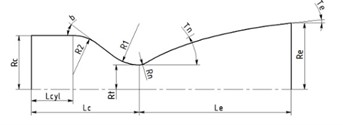
\includegraphics[width=\linewidth]{nozzle_definitions}
	\caption{Definizioni grandezze ugello - RPA }
	\label{fig:nozzle_definitions}
\end{wrapfigure}
In particolare, si introducono i valori di contraction angle $b$, lunghezza caratteristica $L^*$ (o lunghezza camera $L_c$), $R_1/R_t$, $R_n/R_t$ e $R_2/R_{2max}$. Le definizioni sono date in \autoref{fig:nozzle_definitions}. Dopodiché, si sceglie il tipo di modellazione dell'ugello: TIC (truncated ideal contour) o parabolic. Si è optato per una modellazione di ugello parabolico, come precisato anche in  \autoref{subsec:modellazione ugello}. \\
Nel caso di ugello parabolico si definiscono gli angoli $T_n$ e $T_e$ ovvero gli angoli tangenti alla parabola rispettivamente all'inizio e alla fine del divergente. Si definisce infine la percentuale di bell.
\begin{table}[H]
\centering
\begin{tabular}{|c|c|c|c|c|c|c|c|}
\hline
$\bm{L^* \, [m]}$ & $\bm{b \, [\degree]}$ & $\bm{R_1/R_t \, [-]}$ & $\bm{R_n/R_t \, [-]}$ & $\bm{R_2/R_{2,max} \, [-]}$  & $\bm{T_n \, [\degree]}$ &  $\bm{T_e \, [\degree]}$ & $\bm{bell \, [-]}$ \\
\hline
$1$ & $30$ & $1.5$ & $0.382$ & $0.5$ & $31.3109$ & $10.0405$ & $80$\% \\
\hline
\end{tabular}
\caption{Chamber geometry - input}
\label{table:chamb_input}
\end{table}
}

\item \textit{Thermal analysis}: in questa sezione è possibile studiare lo scambio termico impostando diverse tipologie di raffreddamento come regenerative cooling, film e radiation cooling. Questa sezione non è stata utilizzata, prediligendo uno studio del sistema di raffreddamento numerico (\autoref{sec:raffreddamento}).

\item \textit{Propellant feed system}: qui è possibile definire alcune caratteristiche del sistema di alimentazione delle turbopompe. Si definisce il metodo di generazione della potenza (GG o preburner), impostando il funzionamento di tale camera di combustione. In particolare, si definisce il tipo di miscela (fuel o oxidizer rich), temperatura e pressione in camera e perdita di pressione attraverso la camera (\autoref{table:GG_in}).  Si specifica poi il salto di pressione in turbina, la sua efficienza e la sua velocità angolare (\autoref{table:turb_in}). Infine, si definiscono i rami che compongono il sistema. I condotti dell'oxidizer e del fuel sono entrambi composti da un main branch, e dal GG feed branch. Ovvero si riferiscono al condotto di fuel/oxidizer principale e al condotto di spillamento per rifornire la camera del GG (\autoref{table:ox_branch}, \autoref{table:fuel_branch}).\\
In output, si ottengono le grandezze di portata e pressione lungo tutti i condotti appena definiti. In base all'introduzione del tipo di sistema viene anche stimata la nuova performance del motore, influenzata dal sistema di alimentazione introdotto (come visto in \autoref{subsec:analisi performance ciclo a gas}). (Differenze viste in \autoref{table:performance_real} e \autoref{table:performance_eng_real} sul valore $I_s$)

\begin{table}[H]
\centering
\begin{tabular}{|c|c|c|c|}
\hline
\textbf{Type} & $\bm{T_c \, [K]}$ & $\bm{p_c \, [bar]}$ & $\bm{k_{drop} \, [-]}$ \\
\hline
{fuel rich} & $1062.59$ & $67.57$ & $0.966$\\
\hline
\end{tabular}
\caption{GG input data}
\label{table:GG_in}
\end{table}

\begin{table}[H]
\centering
\begin{tabular}{|c|c|c|}
\hline
$\bm{\epsilon \, [-]}$ & $\bm{\eta \, [-]}$ & $\bm{\omega \, [rad/s]}$ \\
\hline
$16.4$ & $0.605$ & $5488$\\
\hline
\end{tabular}
\caption{turbine input data}
\label{table:turb_in}
\end{table}

\begin{table}[H]
\centering
\begin{tabular}{|c|c|c|c|}
\hline
$\bm{p_{in,pump} \, [bar]}$ & $\bm{v_{in,pump} \, [m/s]}$ & $\bm{\dot{m}_{ox,gg}/\dot{m}_{ox} \, [-]}$ & $\bm{A_{in,gg}/A_{in,main} \, [-]}$ \\
\hline
$4.48$ & $5$ & $0.012$ & $0.3$\\
\hline
\end{tabular}
\caption{Oxidizer branch}
\label{table:ox_branch}
\end{table}

\begin{table}[H]
\centering
\begin{tabular}{|c|c|c|c|}
\hline
$\bm{p_{in,pump} \, [bar]}$ & $\bm{v_{in,pump} \, [m/s]}$ & $\bm{\dot{m}_{f,gg}/\dot{m}_{f} [-]}$ & $\bm{A_{in,gg}/A_{in,main} \, [-]}$ \\
\hline
$3.10$ & $5$ & $0.067$ & $0.3$\\
\hline
\end{tabular}
\caption{Fuel branch}
\label{table:fuel_branch}
\end{table}

\end{itemize}

\textbf{Output RPA}

\begin{table}[H]
\centering
\begin{tabular}{|c|c|c|c|c|c|}
\hline
& \textbf{Injector} & \textbf{Nozzle inlet} & \textbf{Nozzle throat} & \textbf{Nozzle exit} & \textbf{Unit} \\
\hline
\textbf{p} & $7.7566$ & $5.9496$ & $3.9690$ & $0.0427$ & \text{MPa} \\
\hline
\textbf{T} & $3569.9063$ & $3498.7671$ & $3344.5972$ & $1473.2666$ & \text{K} \\
\hline
$\bm{c_p}$ & $4.7323$ & $4.7034$ & $0.3706$ & $0.3678$ & \text{kJ/kgK} \\
\hline
$\bm{\gamma}$ & $1.1777$ & $1.1756$ & $1.1716$ & $1.2521$ & \text{-} \\
\hline
\textbf{MM} & $22.2095$ & $22.2541$ & $22.4347$ & $22.6040$ & \text{lb/mol} \\
\hline
\textbf{M} & $0$ & $0.5137$ & $1$ & $3.6856$ & \text{-} \\
\hline
\end{tabular}
\caption{Proprietà termodinamiche in output da RPA - sezione performance analysis }
\label{table:valori RPA sezione performance analysis}
\end{table}

\begin{table}[H]
\centering
\begin{tabular}{|c|c|c|c|}
\hline
\textbf{Parameter}& \textbf{Sea Level} & \textbf{Optimum Exp.} & \textbf{Vacuum}  \\
\hline
$\bm{c^*} \, [m/s]$ & $-$ & $1781.26$ & $-$  \\
\hline
$\bm{u_e} \, [m/s]$ & $2669.97$ & $2915.20$ & $3093.70$ \\
\hline
$\bm{I_s} \, [s]$ & $272.26$ & $297.27$ & $315.47$ \\
\hline
$\bm{c_T} \, [-]$ & $1.4989$ & $1.6366$ & $1.7368$ \\
\hline
\end{tabular}
\caption{Performance reali stimate endoreattore - con $\eta_{reaz} = 0.9856$, $\eta_{nozzle} = 0.9765$ , $\eta_{tot} = 0.9624$}
\label{table:performance_real}
\end{table}

\begin{table}[H]
\centering
\begin{tabular}{|c|c|c|}
\hline
$\bm{I_s \; vac} \, [s]$ & $\bm{I_s \; opt} \, [s]$ & $\bm{I_s \; SL} \, [s]$ \\
\hline
$305.82$ & $288.19$ & $263.97$ \\
\hline
\end{tabular}
\caption{Performance reali stimate motore - da notare le differenze rispetto a \autoref{table:performance_real} su $I_s$}
\label{table:performance_eng_real}
\end{table}



\vspace{10pt}

\begin{table}[H]
\centering
\begin{tabular}{|c|c|c|c|c|}
\hline
& $\bm{\dot{m} \, [kg/s]}$ & $\bm{p_{in} \, [MPa]}$ & $\bm{p_{out} \, [MPa]}$ \\
\hline
\textbf{Inlet} & $1769.26$ & $0.448$ & $0.375$ \\
\hline
\textbf{Pump} & $1769.26$ & $0.375$ & $8.627$ \\
\hline
\textbf{Injector} & $1756.218$ & $8.257$ & $7.757$ \\
\hline
\end{tabular}
\caption{Sistema di alimentazione LOX}
\label{table:Sistema di alimentazione LOX}
\end{table}

\begin{table}[H]
\centering
\begin{tabular}{|c|c|c|c|c|}
\hline
& $\bm{\dot{m} \, [kg/s]}$ & $\bm{p_{in} \, [MPa]}$ & $\bm{p_{out} \, [MPa]}$ \\
\hline
\textbf{Inlet} & $842.974$ & $0.310$ & $0.256$ \\
\hline
\textbf{Pump} & $842.974$ & $0.256$ & $8.519$ \\
\hline
\textbf{Injector} & $773.818$ & $8.257$ & $7.757$ \\
\hline
\end{tabular}
\caption{Sistema di alimentazione RP-1}
\label{table:Sistema di alimentazione RP-1}
\end{table}
Per \autoref{table:Sistema di alimentazione LOX} e \autoref{table:Sistema di alimentazione RP-1} si precisa che la differenza di portata tra sezione pump e injector equivale alla portata spillata per alimentare il GG. Inoltre, le differenze di pressione nelle due tabelle tra sezione 'out' pump e sezione 'in' injector sono date dalle perdita di carico introdotte principalmente da una valvola e il tubo di alimentazione. Si nota anche che per ogni elemento o sezione, sono presenti due valori di pressione (in e out), questo per considerare che viene introdotta una perdita di carico per ogni elemento.

\begin{table}[H]
\centering
\begin{tabular}{|c|c|c|c|c|c|}
\hline
& $\bm{\dot{m} \, [kg/s]}$ & $\bm{p_{in} \, [MPa]}$ & $\bm{p_{out} \, [MPa]}$ & $\bm{T_{in} \, [K]}$ & $\bm{T_{out} \, [K]}$ \\
\hline
\textbf{GG} & $82.198$ & $6.757$ & $6.527$ & $1061.897$ &  $1061.897$\\
\hline
\textbf{Turbine} & $82.198$ & $6.527$ & $0.401$ & $1061.897$ &  $642.453$\\
\hline
\end{tabular}
\caption{Sistema di potenza}
\label{table:sistema_potenza}
\end{table}

\pagebreak
